\chapter{Cơ sở lý luận}
% \addcontentsline{toc}{chapter}{Mở đầu}

\section{Trí tuệ nhân tạo (Artificial Intelligence – AI)}
(\cite{nguyen2018tri})
\subsection{Định nghĩa AI}
\subsection{Thực trạng nghiên cứu lĩnh vực AI}
\subsection{Các xu hướng phát triển AI}
\subsection{Trí tuệ nhân tạo trong giáo dục}
(\cite{garito1991artificial})
(\cite{beck1996applications})
(\cite{goksel2019artificial})
(\cite{devedvzic2004web})

\section{Nền tảng Chatbot}
\subsection{Chatbot là gì?}\par
Tại sao Chatbot được xem là AI?\par
(\cite{bii2013chatbot})

\subsection{Ứng dụng của Chatbot trong giáo dục}
(\cite{10.1007/978-3-030-01689-0_23})
(\cite{hoang2011ung})
(\cite{hsu2012mobile})

\subsection{Nền tảng Chatfuel}

\section{Lý thuyết ứng đáp câu hỏi}
Lý thuyết Ứng đáp Câu hỏi (Item Response Theory - IRT) là một lý thuyết của khoa học về đo lường trong giáo dục, ra đời từ nửa sau của thế kỷ XX và phát triển mạnh mẽ cho đến nay. Trước đó, Lý thuyết Trắc nghiệm cổ điển (Clasical Test Theory – CTT), ra đời từ khoảng cuối thế kỷ XIX và hoàn thiện vào khoảng thập niên 1970, đã có nhiều đóng góp quan trọng cho hoạt động đánh giá trong giáo dục, nhưng cũng thể hiện một số hạn chế. Các nhà tâm lý học (psychometricians) cố gắng xây dựng một lý thuyết hiện đại sao cho khắc phục được các hạn chế đó. Lý thuyết trắc nghiệm hiện đại được xây dựng dựa trên mô hình toán học, đòi hỏi nhiều tính toán, nhưng nhờ sự tiến bộ vượt bậc của công nghệ tính toán bằng máy tính điện tử vào cuối thế kỷ XX – đầu thế kỷ XXI, nên nó đã phát triển nhanh chóng và đạt được những thành tựu quan trọng.\par
Trong phần này, ta quy ước gọi một con người có thuộc tính cần đo lường là thí sinh (person – TS) và một đơn vị của công cụ để đo lường (test) là câu hỏi (item – CH). Để đơn giản hóa cho mô hình nghiên cứu xuất phát có thể đưa ra các giả thiết sau đây:\par
\begin{itemize}
	\item Tính đơn chiều: \textit{Năng lực tiềm ẩn} (latent trait) cần đo chỉ có một chiều (unidimensionality), hoặc ta chỉ đo một chiều của năng lực đó.
	\item Tính độc lập: Các CH là \textit{độc lập địa phương} (local independence), tức là việc trả lời một CH không ảnh hưởng đến các CH khác.
\end{itemize}
Khi thỏa mãn hai giả thiết nêu trên thì không gian năng lực tiềm ẩn đầy đủ chỉ chứa một năng lực. Khi đó, người ta giả định là có một \textit{hàm đặc trưng câu hỏi} (Item Characteristic Function – ICF) phản ánh mối quan hệ giữa các biến không quan sát được (năng lực của TS) và các biến quan sát được (việc trả lời CH). Đồ thị biểu diễn hàm đó được gọi là \textit{đường cong đặc trưng câu hỏi} (Item Characteristic Curve – ICC).
\subsection{Mô hình đường cong đặc trưng câu hỏi đơn chiều, nhị phân, một tham số (mô hình Rasch)}
CH nhị phân là CH mà câu trả lời chỉ có 02 mức: 0 (sai) và 1 (đúng). Mô hình Rasch chỉ biểu diễn CH qua tham số \textit{độ khó} của CH. Phát biểu sau đây của Rasch có giá trị như một tiền đề làm cơ sở cho mô hình của ông:
\begin{flushright}
\textit{"Một người có năng lực cao hơn một người khác thì xác suất để người đó trả lời đúng một câu hỏi bất kì phải lớn hơn xác suất của người sau; cũng tương tự như vậy, một câu hỏi khó hơn một câu hỏi khác có nghĩa là xác suất để một người bất kì trả lời đúng câu hỏi đó phải bé hơn xác suất để trả lời đúng câu hỏi sau."}\\(\cite{rasch1993probabilistic})
\end{flushright}
Với phát biểu trên, có thể thấy xác suất để một TS trả lời đúng một CH nào đó phụ thuộc vào tương quan giữa năng lực của TS và độ khó của CH. Chọn $\Theta$ để biểu diễn năng lực của TS, và $\beta$ để biểu diễn độ khó của CH. Gọi $P$ là xác suất trả lời đúng CH, xác suất đó sẽ phụ thuộc vào tương quan giữa $\Theta$ và $\beta$ theo một cách nào đó, do vậy ta có thể biểu diễn:
\begin{equation}\label{eqn:eqn1-f(P)}
	f(P)=\frac{\Theta}{\beta}
\end{equation}
trong đó $f$ là một hàm nào đó của xác suất trả lời đúng.\par
Lấy logarit tự nhiên của (\ref{eqn:eqn1-f(P)}) ta được:
\begin{equation}\label{eqn:eqn2-lnf(P)}
	\ln f(P)=\ln\left(\frac{\Theta}{\beta}\right)=\ln\Theta-\ln\beta=\theta-b
\end{equation}
Tiếp đến, để đơn giản, khi xét mô hình trắc nghiệm nhị phân, Rasch chọn hàm $f$ chính là biểu thức \textit{mức được thua} (odds) hoặc \textit{khả năng thực hiện đúng} (likelyhood ratio), tức là $f(P)=\frac{P}{1-P}$, qua đó biểu diễn tỉ số của khả năng xảy ra sự kiện khẳng định so với khả năng xảy ra sự kiện phủ định. Như vậy:
\begin{equation}\label{eqn:eqn3-lnP/(1-P)}
	\ln\frac{P}{1-P}=\theta-b
\end{equation}
Từ (\ref{eqn:eqn3-lnP/(1-P)}) ta có thể viết $$\frac{P}{1-P}=\mathbf{e}^{\theta-b}.$$
Suy ra
\begin{equation}\label{eqn:eqn4-P(theta)}
	P(\theta)=\frac{\mathbf{e}^{\theta-b}}{1+\mathbf{e}^{\theta-b}}
\end{equation}
Biểu thức (\ref{eqn:eqn4-P(theta)}) chính là hàm đặc trưng của mô hình ứng đáp CH một tham số, hay còn gọi là \textit{mô hình Rasch}, ta có thể biểu diễn như hình \ref{fig:P(theta)} (khi cho $b=0$):
\begin{figure}[h]\centering\footnotesize
	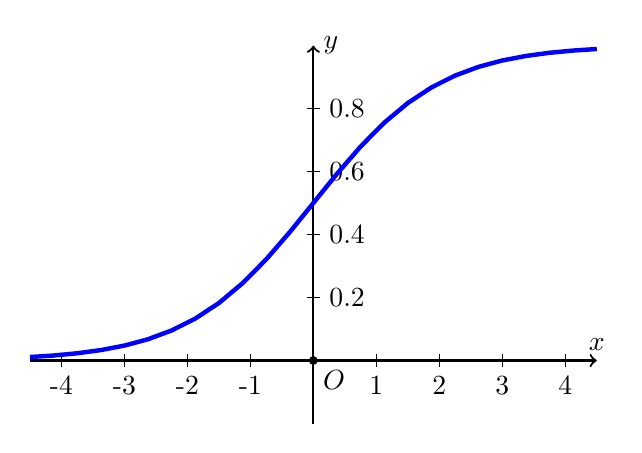
\begin{tikzpicture}[scale=0.8]
		% Oxy system
		\draw [thick, ->] (-4.5, 0) -- (4.5,0) node [above] {$x$};
		\draw [thick, ->] ( 0  ,-1) -- (0  ,5) node [right] {$y$};
		\fill (0,0) circle [radius=2pt] node [below right] {$O$}; % O point
		% Numbering on axist
		\foreach \x in {-4,-3,-2,-1,1,2,3,4}
			\draw (\x,0.1) -- (\x,-0.1) node [below] {\x};
		\foreach \x in {0.2,0.4,0.6,0.8}
			\draw (-0.1,5*\x) -- (0.1,5*\x) node [right] {\x};
		% Graph
		\draw [ultra thick, domain=-4.5:4.5, blue] plot (\x, {5 * exp(\x) / (1+exp(\x))});
	\end{tikzpicture}
	\caption{Đồ thị ICC một tham số (mô hình Rasch)}
	\label{fig:P(theta)}
\end{figure}\par

\subsection{Ước lượng các tham số của câu hỏi trắc nghiệm}
\subsection{Điểm thực – đường cong đặc trưng của đề trắc nghiệm}
\subsection{Ước lượng năng lực của thí sinh}
% Có nhiều định nghĩa khác nhau về đo lường, nhìn từ các góc độ khác nhau. Ta lưu ý đến hai định nghĩa sau: \textit{Đo lường là gán các con số vào các cá thể theo một quy tắc có hệ thống để biểu diễn các đặc tính của các cá thể đó} (\cite{allen2001introduction}) và \textit{Một số đo là một vị trí trên một đường. Đo lường là quá trình cấu trúc các đường và định vị các cá thể trên các đường đó.} (\cite{wright1979best}).\par

(\cite{thiep2011do})

% Using \texttt{biblatex} you can display bibliography divided into sections, 
% depending of citation type. 
% Let's cite! Einstein's journal paper \cite{bai-bao-1} and the Dirac's 
% book \cite{sach-1} are physics related items. 
% Next, \textit{The \LaTeX\ Companion} book \cite{website-1}, the Donald Knuth's website \cite{sach-2}; but the others Donald Knuth's items \cite{bai-bao-1} are dedicated to programming.
